\section{The advantages of combining resolution and precision}
\label{sec:motivation}

Traditional data reduction techniques work by either truncating the finest few resolution levels, or
truncating the last few low-ordered bits of every sample, but rarely both. Our aim in this section
is to show that significant gain can be achieved when one combines both dimensions, namely
resolution and precision, for data reduction. To do so, for each data set, we construct and compare
three different streams, which use different sorting criteria to sort the same set of chunks in
decreasing order of weights. We will use $W(c)$ to denote a sorting criteria, which is any function
that takes a chunk, $c$, and returns its `'weight'', which determines how important the chunk is.

We compare the three streams by plotting an error curve for each, with regards to three error
metrics, namely root-mean-square error (Figure \ref{fig:motivation-rmse}), histogram error (Figure
\ref{fig:motivation-histogram}), and isocontour error (Figure \ref{fig:motivation-isocontour}). For
each metric, the function is reconstructed every time a new chunk is received from a stream, then
the relevant quantity (the function itself, its histogram, or an isocontour) is computed from the
reconstructed function, and compared against the same quantity computed from the original (lossless)
function. The definitions of histogram error and isocontour error are discussed in detail in Section
[REF] and Section [REF] respectively.

\begin{figure}[h]
  \centering
	\subcaptionbox{Boiler}
  {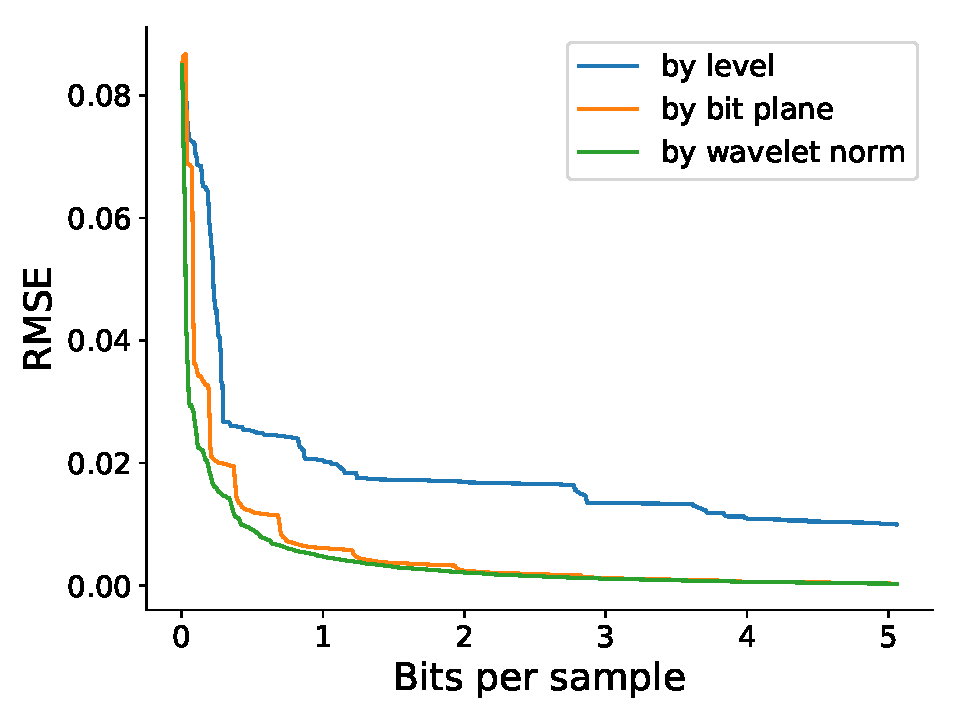
\includegraphics[width=0.48\linewidth]{img/motivation/motivation-psnr-boiler.pdf}}
	\subcaptionbox{Diffusivity}
 	{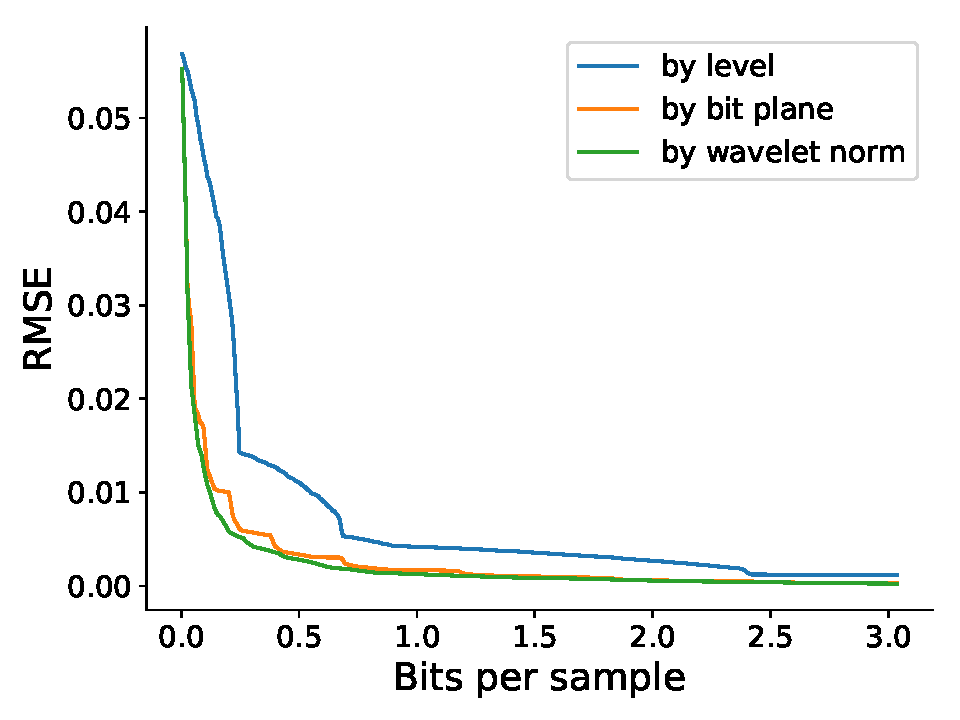
\includegraphics[width=0.48\linewidth]{img/motivation/motivation-psnr-diffusivity.pdf}}
	\subcaptionbox{Euler}
 	{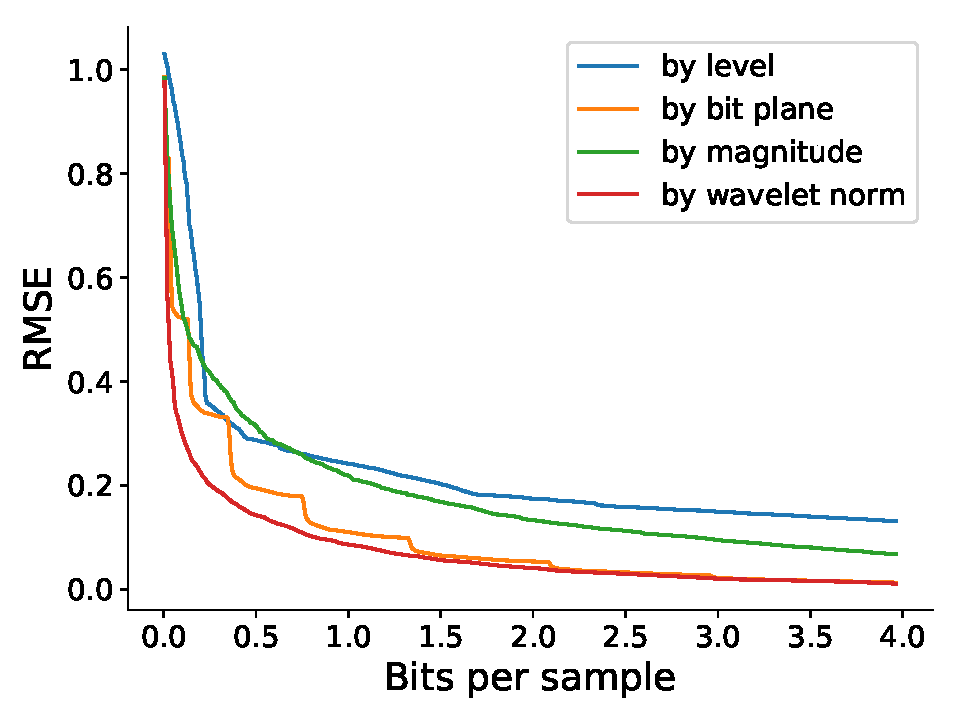
\includegraphics[width=0.48\linewidth]{img/motivation/motivation-psnr-plasma.pdf}}
	\subcaptionbox{Turbulence}
 	{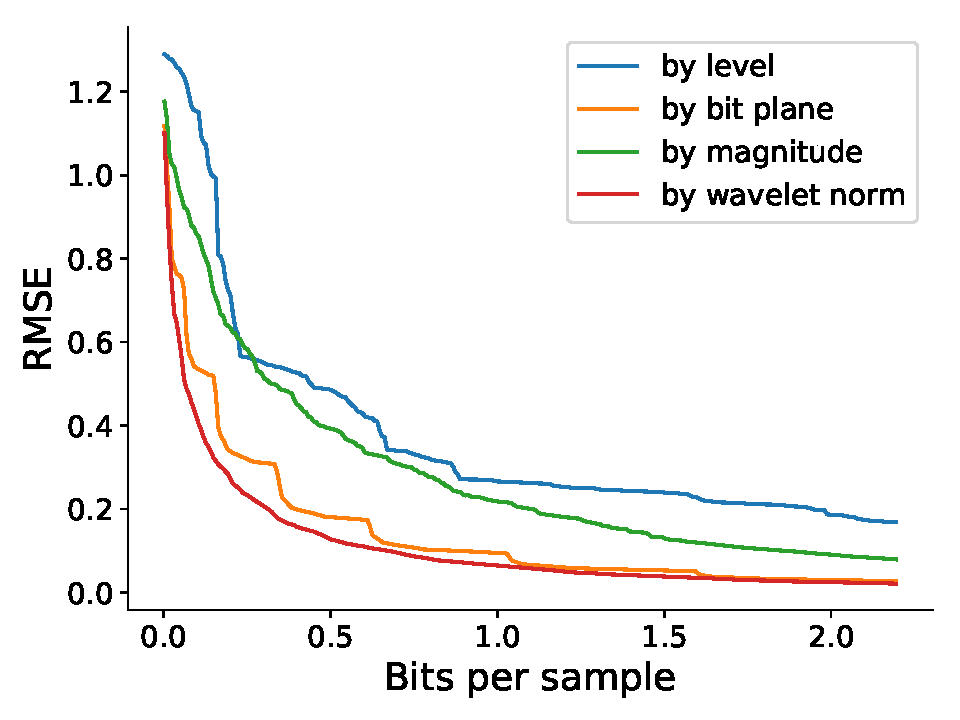
\includegraphics[width=0.48\linewidth]{img/motivation/motivation-psnr-turbulence.pdf}}
	\subcaptionbox{Plasma}
 	{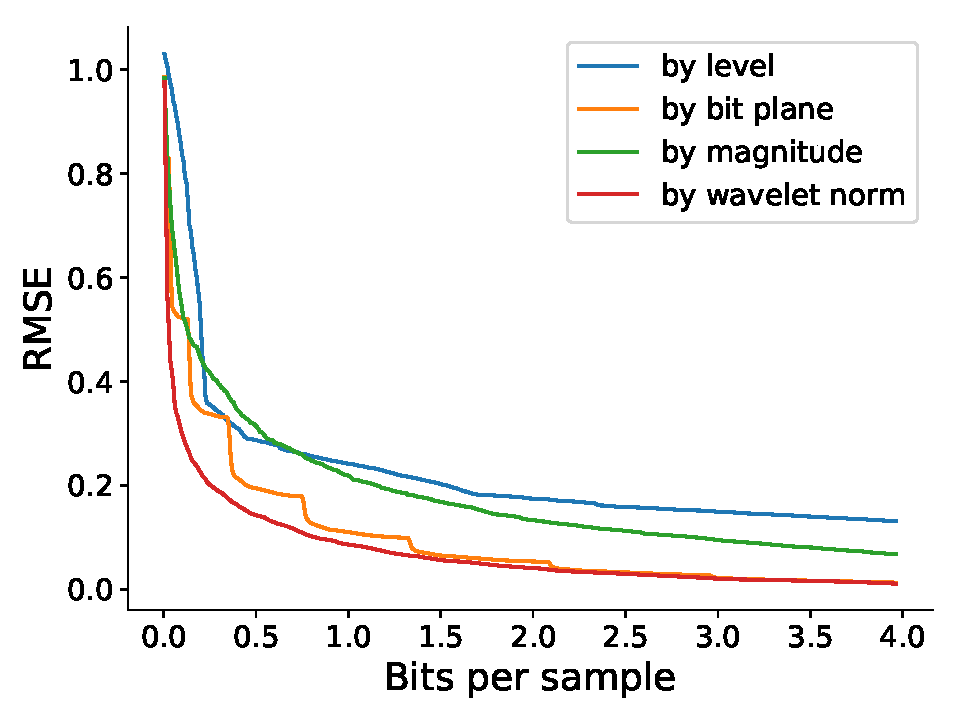
\includegraphics[width=0.48\linewidth]{img/motivation/motivation-psnr-plasma.pdf}}
	\subcaptionbox{Velocity-z}
 	{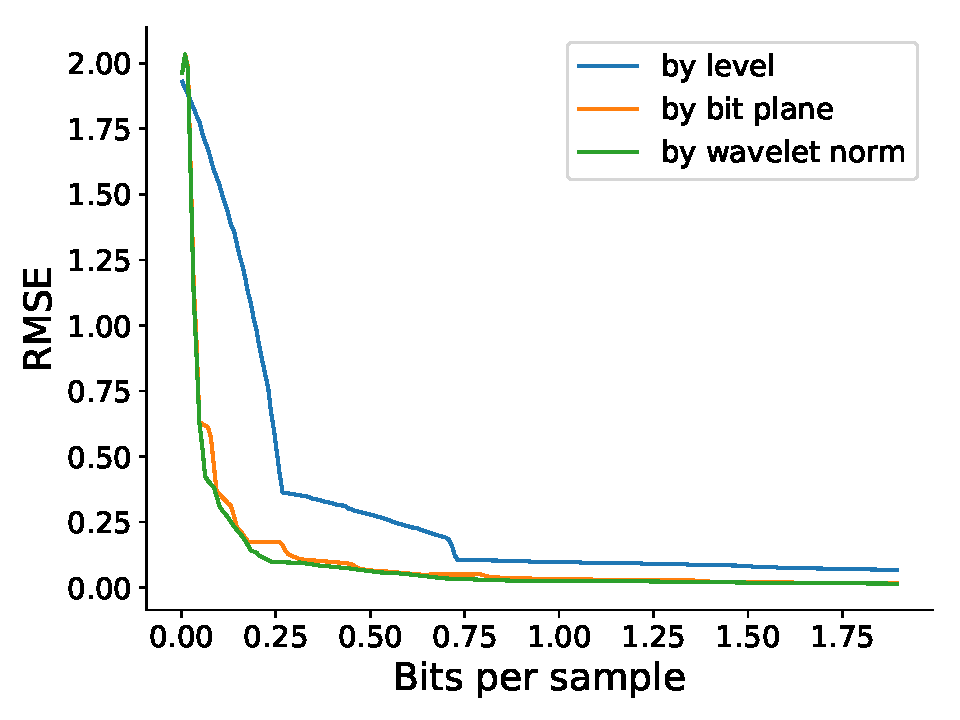
\includegraphics[width=0.48\linewidth]{img/motivation/motivation-psnr-velocityz.pdf}}
 	\caption{Root-mean-square error of reconstructed functions using the three data-agnostic streams
 	defined in Section \ref{sec:motivation}. Lower is better. The streams are truncated to highlight
 	the differences, without omitting important information. \emph{by wavelet norm} performs best,
 	followed closely by \emph{by bit plane}.}
 	\label{fig:motivation-rmse}
\end{figure}

\begin{figure}[h]
  \centering
	\subcaptionbox{Boiler}
  {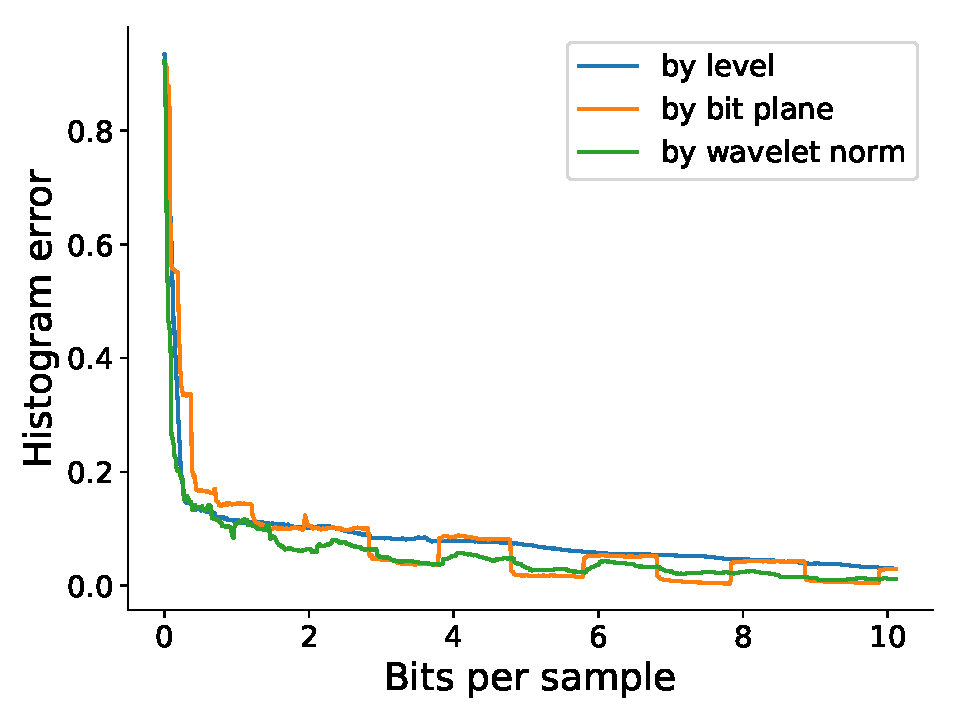
\includegraphics[width=0.48\linewidth]{img/motivation/motivation-histogram-boiler.pdf}}
	\subcaptionbox{Diffusivity}
 	{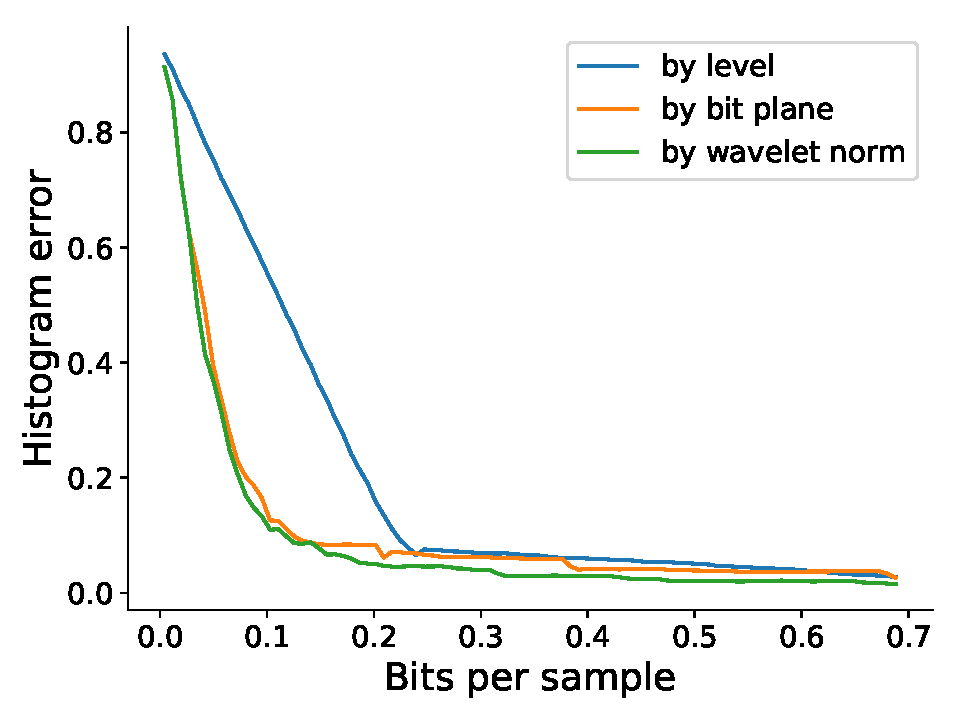
\includegraphics[width=0.48\linewidth]{img/motivation/motivation-histogram-diffusivity.pdf}}
	\subcaptionbox{Euler}
 	{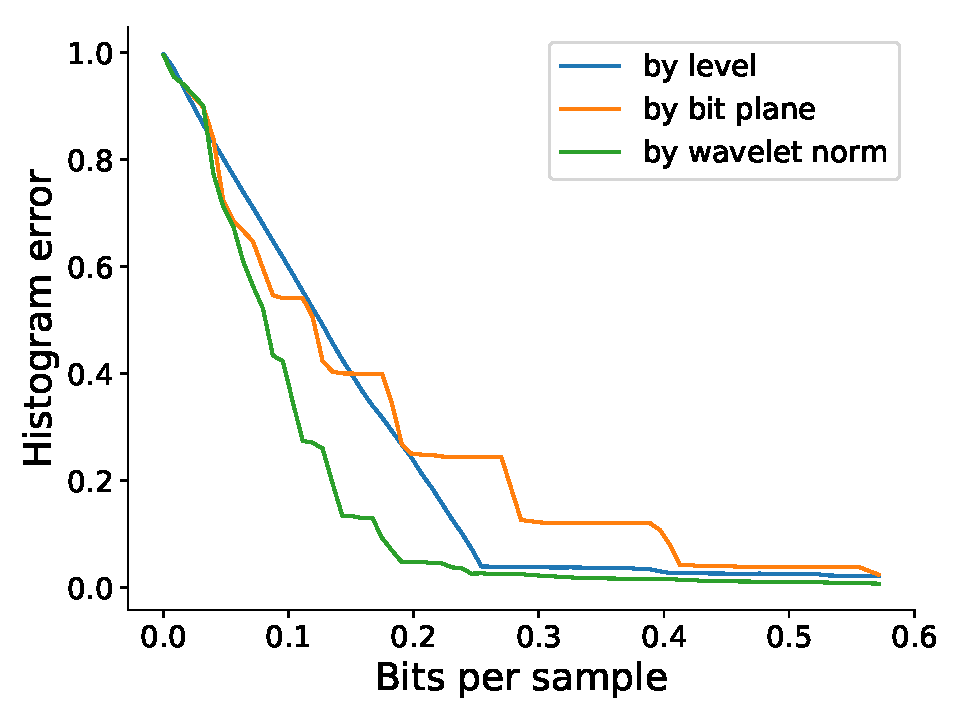
\includegraphics[width=0.48\linewidth]{img/motivation/motivation-histogram-euler.pdf}}
	\subcaptionbox{Turbulence}
 	{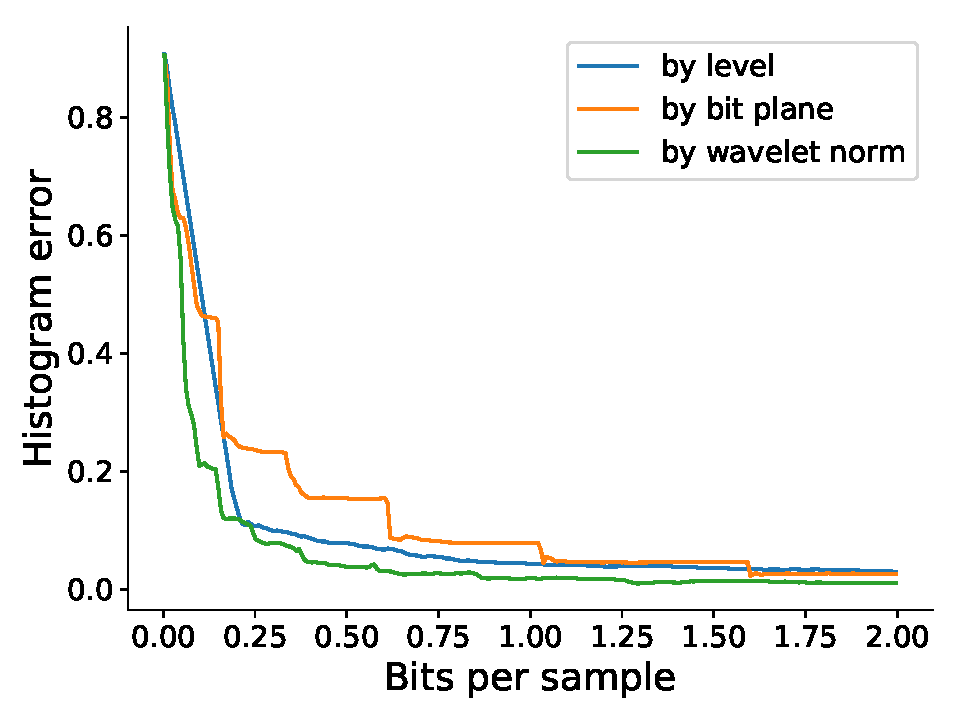
\includegraphics[width=0.48\linewidth]{img/motivation/motivation-histogram-turbulence.pdf}}
	\subcaptionbox{Plasma}
 	{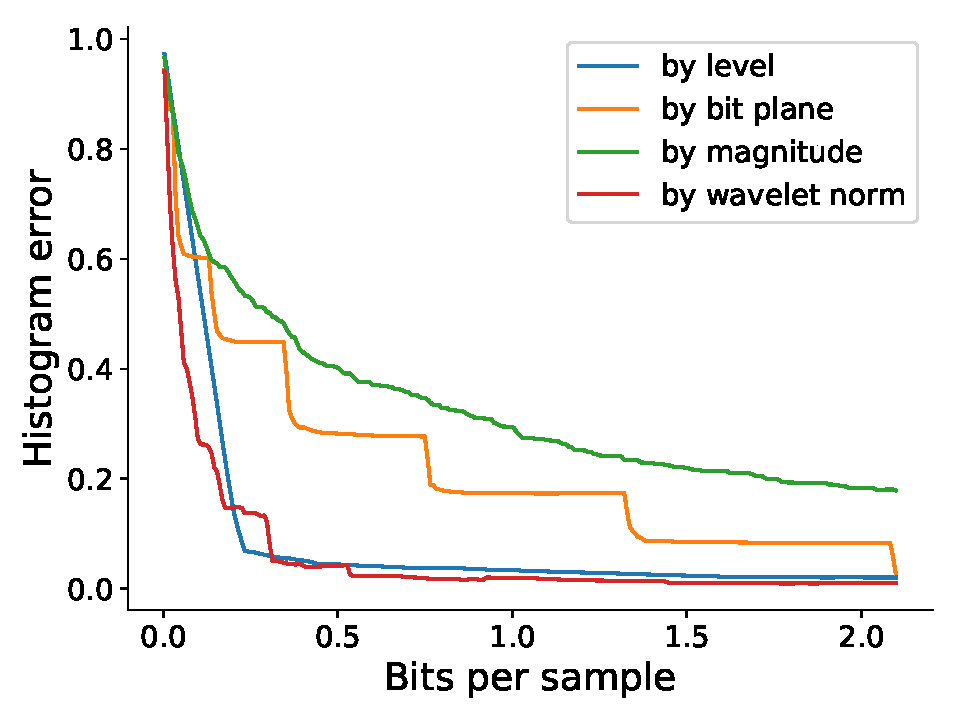
\includegraphics[width=0.48\linewidth]{img/motivation/motivation-histogram-plasma.pdf}}
	\subcaptionbox{Velocity-z}
 	{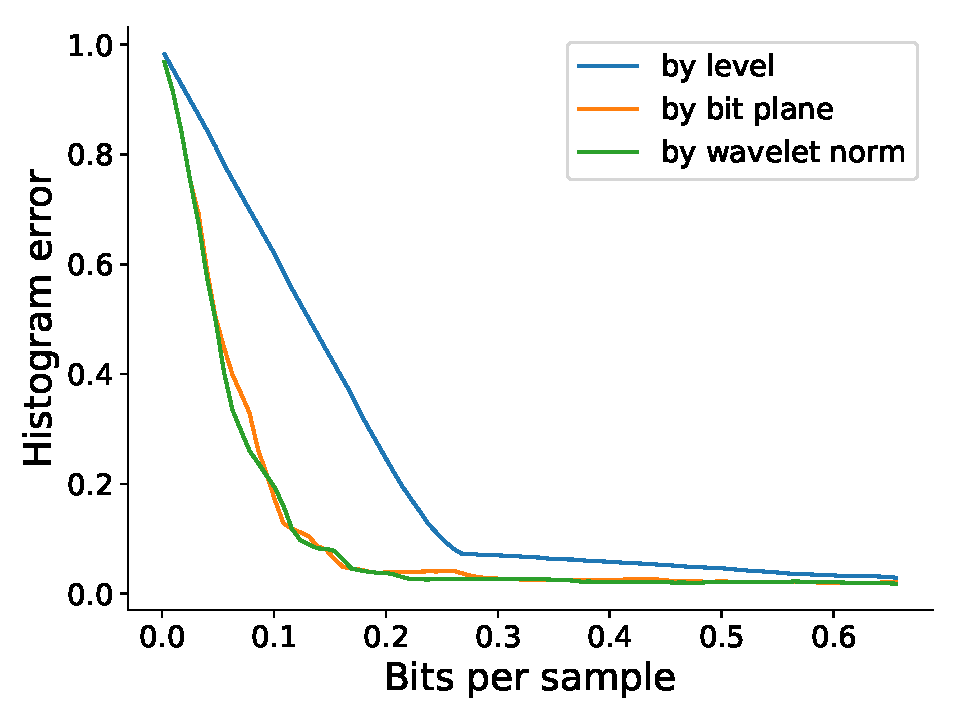
\includegraphics[width=0.48\linewidth]{img/motivation/motivation-histogram-velocityz.pdf}}
 	\caption{Histogram error of reconstructed functions using the three data-agnostic streams defined
 	in Section \ref{sec:motivation}. Lower is better. Each histogram comprises of 256 bins. The
 	streams are truncated to highlight the differences, without omitting important information.
 	\emph{by wavelet norm} performs best.}
 	\label{fig:motivation-histogram}
\end{figure}

\begin{figure}[h]
  \centering
	\subcaptionbox{Boiler, isovalue = $0.07$}
  {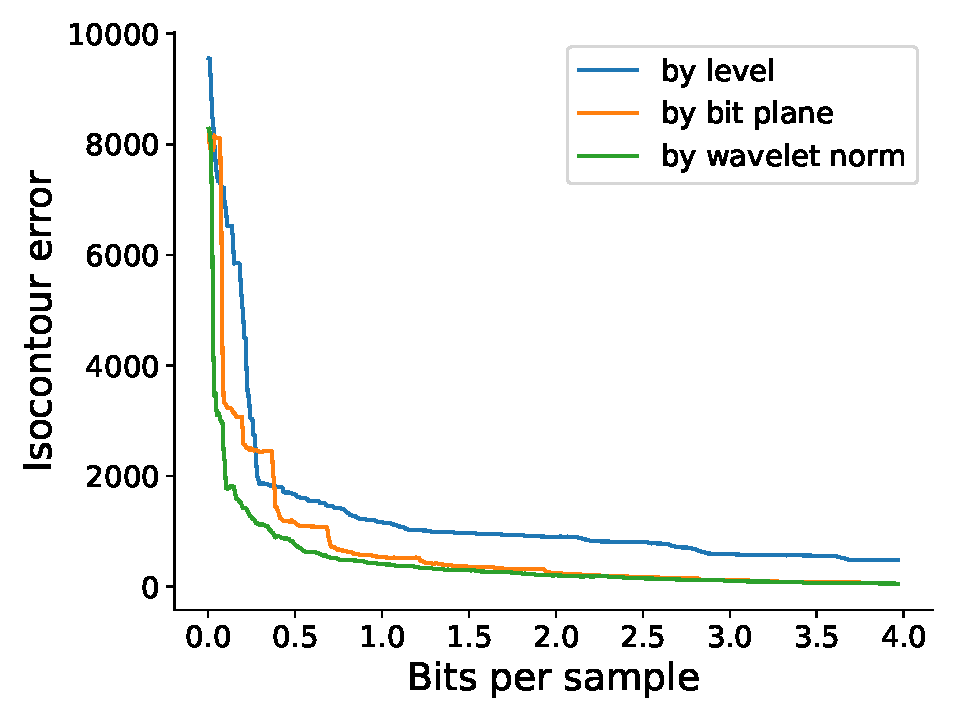
\includegraphics[width=0.48\linewidth]{img/motivation/motivation-isocontour-boiler.pdf}}
	\subcaptionbox{Diffusivity, isovalue = $0.04315$}
 	{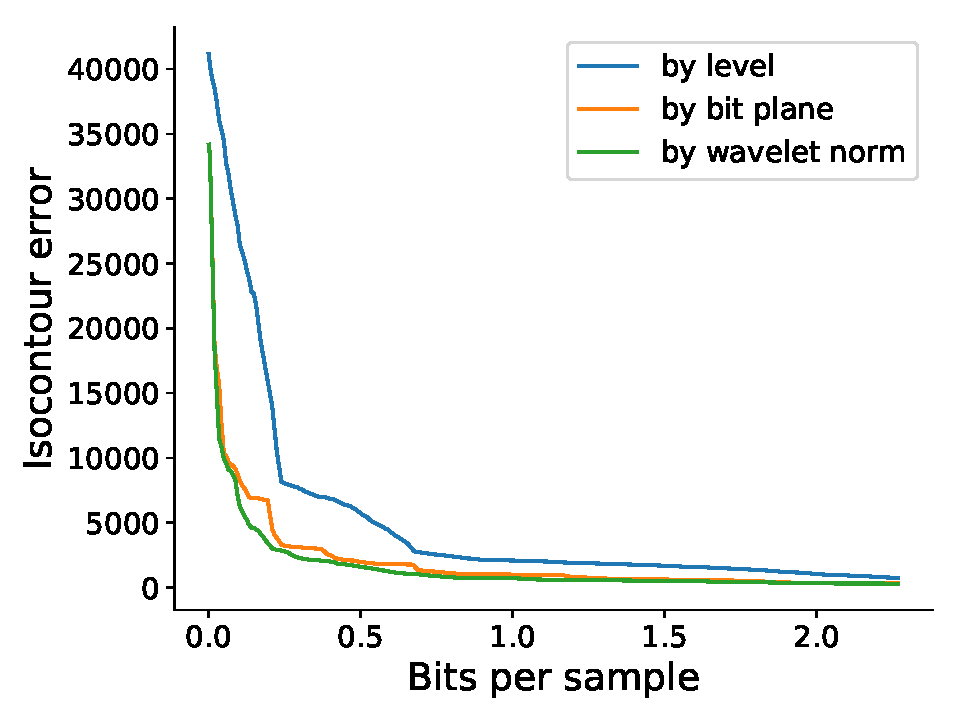
\includegraphics[width=0.48\linewidth]{img/motivation/motivation-isocontour-diffusivity.pdf}}
	\subcaptionbox{Euler, isovalue = $3$}
 	{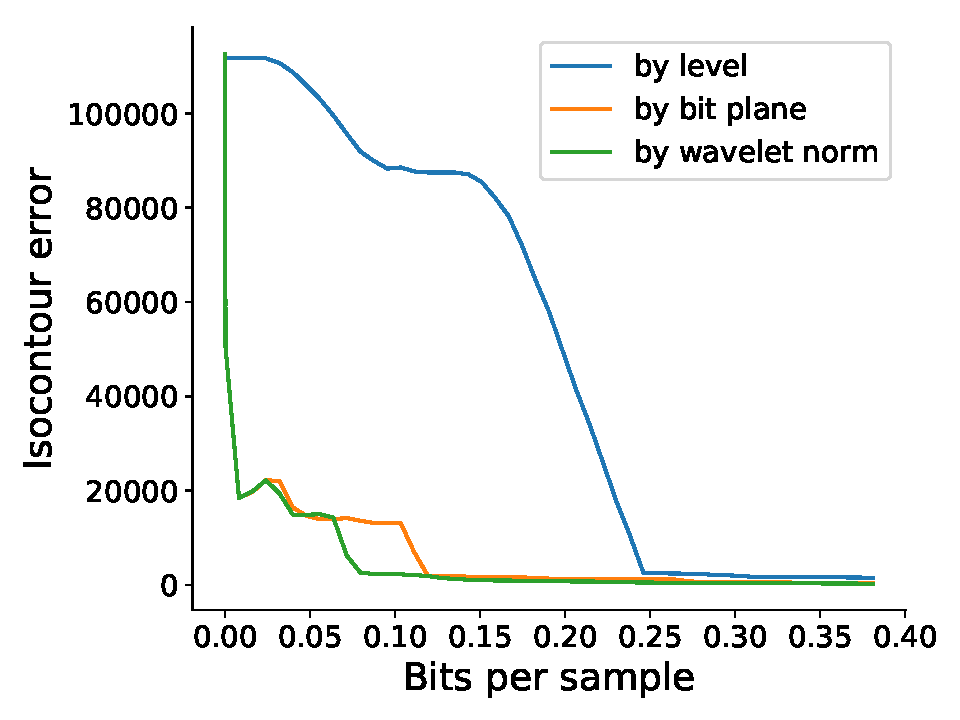
\includegraphics[width=0.48\linewidth]{img/motivation/motivation-isocontour-euler.pdf}}
	\subcaptionbox{Turbulence, isovalue = $2$}
 	{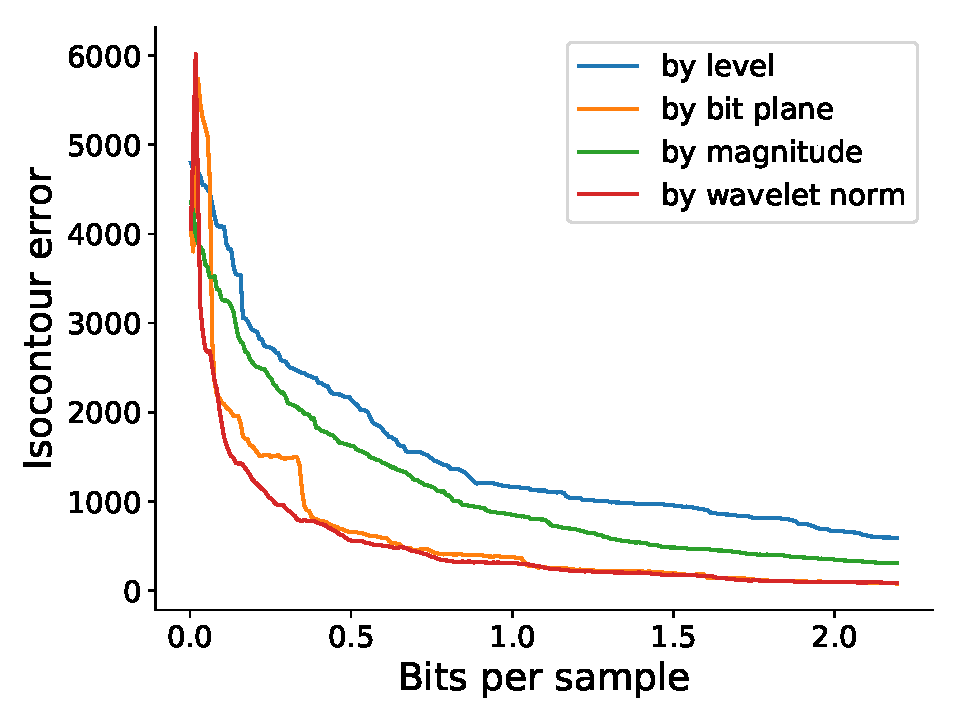
\includegraphics[width=0.48\linewidth]{img/motivation/motivation-isocontour-turbulence.pdf}}
	\subcaptionbox{Plasma, isovalue = $2$}
 	{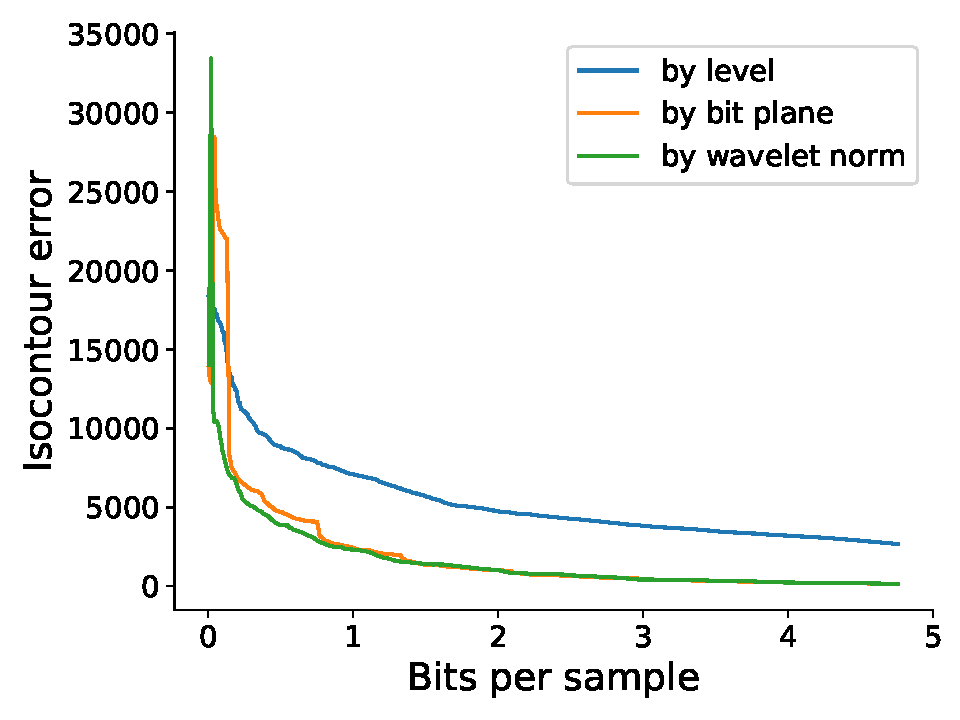
\includegraphics[width=0.48\linewidth]{img/motivation/motivation-isocontour-plasma.pdf}}
	\subcaptionbox{Velocity-z, isovalue = $-2$}
 	{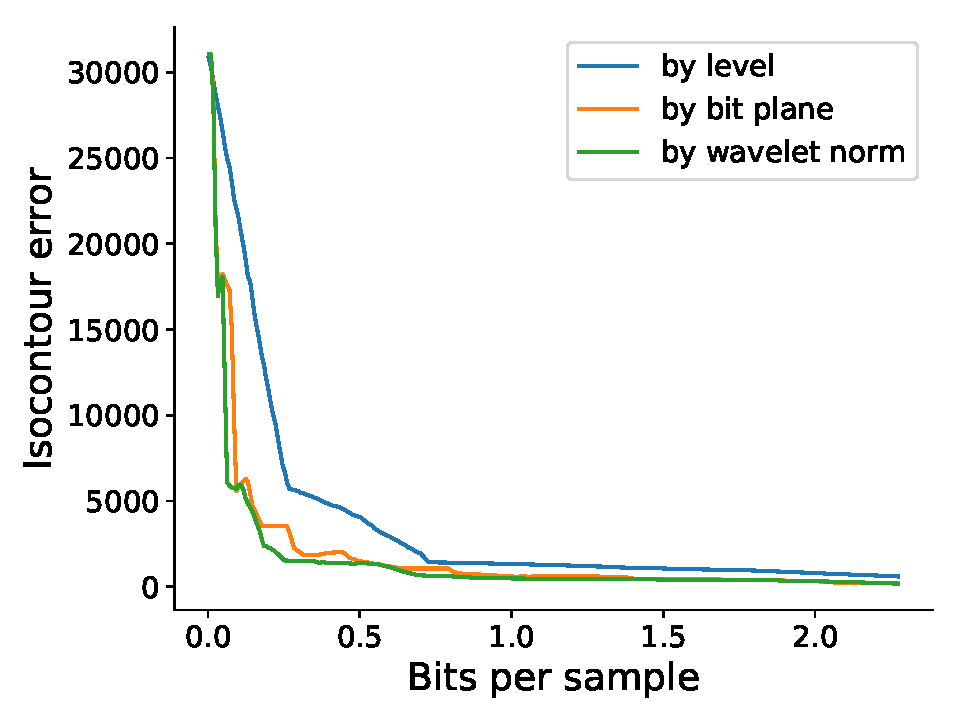
\includegraphics[width=0.48\linewidth]{img/motivation/motivation-isocontour-velocityz.pdf}}
 	\caption{Isocontour error of reconstructed functions using the three data-agnostic streams defined
 	in Section \ref{sec:motivation}. Lower is better. The streams are truncated to highlight the
 	differences, without omitting important information. \emph{by wavelet norm} performs best.}
 	\label{fig:motivation-isocontour}
\end{figure}

It can be seen that, for all metrics, the \emph{by wavelet norm} stream consistently performs the
best. The \emph{by bit plane} works almost as well as \emph{by wavelet norm} for RMS error and
isocontour error, but not for histogram error. \emph{by level} works poorly in almost all cases.
These results show that it is often suboptimal to stream or reduce data exclusively in either
resolution or precision. Combining these two dimensions of data reduction can lead to significant
quality improvement at the same bit rate, especially when quantities of interest other than simply
the function itself are considered. The reason is that \emph{by wavelet norm} can take advantage of
the fact that a higher-ordered bit from a fine-scale coefficient could contribute more than a
lower-ordered bit from a coarse-scale coefficient (which \emph{by level} ignores), and vice-versa
(which \emph{by bit plane} ignores). It is unclear, however, whether \emph{by wavelet norm} is the
best stream to use in all cases. To answer this question, we will expand our study from
data-agnostic to data-dependent streams that are optimized for each of these quantities of interest.
While data-dependent streams are likely unrealizable in practice due to the fact that the
`'receiver'' of data does not have access to the data beforehand, we hope they provide insights for
designing streams that improve on the generic \emph{by wavelet norm}, by being tailored to each
error metric.

\subsection{Data-dependent, quantity-optimized streams}
\label{sec:data_dep_streams}

This section aims to solve the problem of finding the most optimal (and data-dependent) stream
possible, given a data set and an error metric. An error metric is a function $E(Q(f'),Q(f))$, where
$f$ is the original data field and $f'$ is a reconstructed version of $f$ using a subset of the
bits. $Q$ is an operation that trasnforms a raw data fields (e.g., $f$ and $f'$) to some quantity of
interest (e.g., derivatives, histograms, isocontours, etc). There can be multiple error functions
$E$ that makes sense for the same quantity $Q$. In this paper, we choose to use only one error
metric with each quantity, one which we believe is either common, or intuitive and simple without
sacrificing generalizability. The list of quantity-optimized streams studied in this paper includes
\emph{rmse-optimized} (Section [REF]), \emph{gradient-optimized} (Section [REF]),
\emph{laplacian-optimized} (Section [REF]), \emph{histogram-optimized} (Section [REF]), and
\emph{isocontour-optimized} (Section [REF]).

Studying a (data-dependent) quantity-optimized stream is important because such a stream serves both
as a benchmark, and a source of insights for other, more practical streams for the same quantity.
One way to define the ``optimal'' stream for a quantity $G$ could be the stream that incurs the
minimum error $E$ at every point. However, in trying to realize it, our experience has been that
such a stream does not exist. Assume otherwise that the optimal stream exists, then by its
definition, it must be possible to construct it using the following greedy algorithm: start with a
pool of all the chunks (and correspondingly an all-zero $f'$ and a presumably very high $E$), pick
the chunk that when enabled, would minimize $E$, remove it from the pool. Repeatedly pick the next
chunk that minimizes $E$, until the pool is empty. Running this algorithm, we have noticed that
there can be a situation in which the next chunk that minimizes the error is on a low-order bit
plane of a very fine-scale coefficient, which contributes little to the reconstructed function. The
error is minimized because it is kept approximately constant. In this case it is actually better to
pick a chunk that increases the error, but otherwise contributes a lot more to the reconstructed
function. In optimization terms, it is necessary to move in a direction that increases the error to
avoid getting stuck in a local minima.

The optimal stream for an error metric can also be defined as the stream such that the area bounded
by its plotted error curve and the horizontal axis is smallest. However, the usefulness of such a
definition is limited in practice, because a stream should be able to be terminated at any point and
still be expected to produce as small of an error as possible. Instead, we observe that the greedy
algorithm stated in the paragraph above can be slightly modified to avoid the problem of being stuck
in local minima. We start with a pool consisting of all the chunks and an empty stream, and build
the stream back to front. In each step, the chunk whose removal from the pool has the least impact
on the error $E$ is removed and inserted to the beginning of the current stream. This algorithm
solves the problem of unimportant chunks being picked too early in the original algorithm, because
here, being picked early means they would be at the end of the stream, instead of the beginning.

In our experience, however, the back-to-front greedy algorithm is too costly in practice. Ignoring
all the steps done in each iteration, this algorithm amounts to an $n^2$-iteration, 2-level nested
loop, where $n$ is the number of chunks. In 2D, with a $256^2$ data set, a chunk size that spans
$16$ coefficients, and $16$ bits of quantization, the total number of chunks would be $n=65536$, and
$n^2$ would be in the billions, which we have found to be prohibitively large. We have therefore
adopted a simplified version of this algorithm, where only one pass through the chunks are needed.
Our modified algorithm disables (sets to zero) a new chunk $c_i$ in each iteration, computes and
records the error $E_i$ due to chunk $c_i$ missing, and enables again the chunk at the end of the
iteration. After $n$ iterations, each chunk has an associated weight, $E_i$. The optimal stream,
then, is simply a sorted list of chunks, in decreasing order of the weights. In our experience, this
simplified algorithm brings the running time down from days to minutes, while retaining the same
performance.